%%%%%%%%%%%%%%%%%%%%%%%%%%%%%%%%%%%%%%%%%
% University/School Laboratory Report
% LaTeX Template
% Version 3.1 (25/3/14)
%
% This template has been downloaded from:
% http://www.LaTeXTemplates.com
%
% Original author:
% Linux and Unix Users Group at Virginia Tech Wiki 
% (https://vtluug.org/wiki/Example_LaTeX_chem_lab_report)
%
% License:
% CC BY-NC-SA 3.0 (http://creativecommons.org/licenses/by-nc-sa/3.0/)
%
%%%%%%%%%%%%%%%%%%%%%%%%%%%%%%%%%%%%%%%%%

%----------------------------------------------------------------------------------------
%	PACKAGES AND DOCUMENT CONFIGURATIONS
%----------------------------------------------------------------------------------------

\documentclass{article}
\usepackage[spanish,es-tabla]{babel}
\newcommand\Monthname[1][EMPTY]{%
  \ifnum1=#1Enero\else
  \ifnum2=#1Febrero\else
  \ifnum3=#1Marzo\else
  \ifnum4=#1Abril\else
  \ifnum5=#1Mayo\else
  \ifnum6=#1Junio\else
  \ifnum7=#1Julio\else
  \ifnum8=#1Agosto\else
  \ifnum9=#1Septiembre\else
  \ifnum10=#1Octubre\else
  \ifnum11=#1Noviembre\else
  \ifnum12=#1Diciembre\else
  \fi\fi\fi\fi\fi\fi\fi\fi\fi\fi\fi\fi
}

\usepackage{datetime}

\usepackage[a4paper,
 %left=20mm,
 top=30mm,
 bottom=25mm,
 headheight=80pt,
 headsep=15mm
 ]{geometry}


\usepackage[version=3]{mhchem} % Package for chemical equation typesetting
\usepackage{graphicx} % Required for the inclusion of images

\usepackage{amsfonts}
\usepackage{amsmath} % Required for some math elements 
\usepackage{mathtools}


\DeclarePairedDelimiter{\ceil}{\lceil}{\rceil} %this is for ceil and floor symbols
\DeclarePairedDelimiter{\floor}{\lfloor}{\rfloor} %this is for ceil and floor symbols

\usepackage{changepage} % Required in text margins
\usepackage{xcolor} % Required changing color 
\usepackage{sectsty} %Required to change section headers
\usepackage{titlesec} % Required for section spacing
\usepackage{enumitem}
\usepackage{tocloft} % Better in table of contents
\usepackage[blocks]{authblk}% The option is for block layout
\usepackage[pdfborder={0 0 0}]{hyperref}% For email addresses
\usepackage{fancyhdr} %Required for Headers

\usepackage[nottoc]{tocbibind} %Better to add references and more in table of contents (nottoc is to remove indice in toc)

\usepackage{layout} %Used for "margin debugging"

\usepackage[export]{adjustbox} 
\usepackage{float}

\usepackage{subfig}% http://ctan.org/pkg/subfig


\pagestyle{fancy}
\fancyheadoffset{0cm} %Used for heading without margins
\fancyhead[L]{} % 1. sectionname

\rhead{ \textit{Simulaci\'on y Animaci\'on Biomec\'anica de un Humanoide}}
\renewcommand{\headrulewidth}{0.4pt}


\renewcommand\cfttoctitlefont{\hfill\huge\bfseries\color{cyan}}
\renewcommand\cftaftertoctitle{\hfill\mbox{}}

\setlist{leftmargin=5.5mm}

\titlespacing*{\section} {0pt}{6ex}{2ex}
\titlespacing*{\subsection} {0pt}{4ex}{0.7ex}

\sectionfont{\color{cyan}} % Changing color to section headers
\subsectionfont{\color{cyan}} % Changing color to subsection headers
\subsubsectionfont{\color{cyan}} % Changing color to subsubsection headers

%\setlength\parindent{0pt} % Removes all indentation from paragraphs

\renewcommand{\labelitemi}{$-$}

\renewcommand{\baselinestretch}{1.25} 

\renewcommand{\labelenumi}{\alph{enumi}.} % Make numbering in the enumerate environment by letter rather than number (e.g. section 6)

\let\datespanish\relax
\newdateformat{datespanish}{\Monthname[\THEMONTH] \THEYEAR}

%\usepackage{times} % Uncomment to use the Times New Roman font

%----------------------------------------------------------------------------------------
%	DOCUMENT INFORMATION
%----------------------------------------------------------------------------------------

\title{\textbf{\Large{\\ \underline{PROYECTO} \underline{FINAL} \\ \vspace*{2ex} INGENIER\'IA INFORM\'ATICA - ITBA \\}} \vspace*{4ex} 
\textbf{\textcolor{cyan}{\textit{SIMULACI\'ON Y ANIMACI\'ON BIOMEC\'ANICA \\DE UN HUMANOIDE}  }  \vspace*{3ex}} } % Title

\author{\textbf{Alumnos:} }
\affil{\textbf{Enzo Altamiranda Graterol}\\% If the blocks option of authblk is removed \\ is treated as ,
\url{ealtamir@itba.edu.ar}}

\affil{\textbf{Teresa Fontanella De Santis}\\
\url{tfontane@itba.edu.ar}}

\affil{\textbf{Tom\'as Mehdi}\\
\url{tmehdi@itba.edu.ar}\vspace*{3ex}}

\author{\textbf{Tutor:}}
\affil{ \textbf{Dr. Daniel Ricardo Parisi} \vspace*{8ex}}

\date{\textbf{\small{\today}}} % Date for the report

\author{  \small{\textbf{Instituto Tecnol\'ogico de Buenos Aires - ITBA \\  Departamento de Ingenier\'ia Inform\'atica} }  }
\affil{\vspace*{0ex}}
\begin{document}

% \layout %CAREFUL!! This is only for "debugging"

\maketitle % Insert the title, author and date
\thispagestyle{empty} %Page without number

\newpage
\tableofcontents
\newpage

% If you wish to include an abstract, uncomment the lines below
 \begin{abstract}
 
\addcontentsline{toc}{section}{Resumen} %Including abstract in table of contents
\noindent

\begin{adjustwidth}{1.05cm}{0cm}
Este proyecto tiene como objetivo crear una simulaci\'on y animaci\'on de un humano virtual, con las siguientes propiedades:
\begin{itemize}[leftmargin=5.5mm]
\item Biomec\'anica: que tanto su estructura (peso, altura y posici\'on de cada una de sus partes) como su interacci\'on con el entorno, respondan a comportamientos f\'isicos reales y exactos.
\item Inteligencia Artificial: que aprenda a caminar por s\'i mismo, utilizando para ello m\'etodos de \textit{soft computing} como Algoritmos Gen\'eticos.
\end{itemize}

\end{adjustwidth}

 \end{abstract}

%----------------------------------------------------------------------------------------
%	SECTION 1
%----------------------------------------------------------------------------------------


\section{Introducci\'on}

%\begin{adjustwidth}{1cm}{0cm}
\textbf{No est\'a terminada a\'un} \\Siempre ha sido de inter\'es la simulaci\'on biomec\'anica de seres vivos, especialmente en las ciencias naturales (zoolog\'ia, medicina, etc.). Pero \'ultimamente se ha incrementado el inter\'es en otras \'areas de aplicaci\'on, como los videojuegos, para agregarle  .
Una caracter\'istica muy importante de este trabajo es que, el humanoide no es fruto de una animaci\'on, sino  un objeto compuesto de segmentos f\'isicos, que interaccionan. 
%\end{adjustwidth}


\section{Herramientas}

%\begin{adjustwidth}{1cm}{0cm}
\subsection{Motor F\'isico}

%\begin{adjustwidth}{1.2cm}{0cm}
Se le llama motor f\'isico o \textit{physics engine} a un  ``software capaz de realizar simulaciones de ciertos sistemas f\'isicos, como la din\'amica del cuerpo r\'igido, el movimiento de un fluido y la elasticidad" \cite{wikiPhysicsEngine}. \\
Actualmente, existen muchos motores f\'isicos: ya sea de c\'odigo propietario (PhysX, Havok), como open-source (\textit{Bullet Physics}, \textit{Box2D}, Newton, OGRE). Considerando an\'alisis relacionados \cite{Comparissons}\cite{Comparissons2}, y la necesidad de que el espacio simulado fuese en 3D, se decidi\'o que \textit{Bullet Physics}\cite{LinkBullet} es el m\'as id\'oneo. Est\'a implementado en C++ y ha sido utilizado en varios juegos (\textit{Grand Theft Auto IV} y V, etc); en los efectos especiales de pel\'iculas (Hancock, Bolt, etc.); y proyectos cient\'ificos, como la herramienta open-source \textit{Tensegrity Robotics Toolkit} de la NASA\footnote{http://bulletphysics.org/Bullet/phpBB3/viewtopic.php?f=17\&t=9978}; entre otros.\\
Si bien (como se ver\'a m\'as adelante) Bullet tiene problemas asociados con el coeficiente de restituci\'on, posee una muy buena performance en la detecci\'on de colisiones, la din\'amica y la resoluci\'on de constraints. Esto se debe, en parte, a diferentes algoritmos iterativos de orden lineal (donde el m\'as importante es \textit{Sequential Impulse}), de caching y tambi\'en a la utilizaci\'on de un modelo de fricci\'on de Coulomb aproximado \cite{Catto}. Adem\'as, el motor f\'isico brinda la posibilidad de regular la precisi\'on requerida en estos c\'alculos (sin olvidar que, con iguales recursos, a mayor precisi\'on, mayor capacidad de c\'omputo requerida y, ergo, mayor tiempo). Dado que la construcci\'on del humanoide implica definir caracter\'isticas y restricciones de movimiento de cada una de sus partes, lo antes mencionado fue crucial para la elecci\'on de \textit{Bullet Physics} en este proyecto.

%\end{adjustwidth}
\subsubsection{Modelo de fricci\'on utilizado y su verificaci\'on}

%\begin{adjustwidth}{1.3cm}{0cm}
Hay reglas f\'isicas relacionadas con el entorno y que son muy importantes para la caminata: el modelo de fricci\'on, con sus respectivos coeficientes de fricci\'on y restituci\'on.\\  
En base a los modelos f\'isico-matem\'aticos utilizados  en los dos fen\'omenos en cuesti\'on (y que se explicar\'an a continuaci\'on), y pensando en posibles futuras simulaciones de varios humanoides chocando e interactuando entre s\'i; se llevaron a cabo dos experimentos para verificar que estuvieran en concordancia con los datos arrojados por \textit{Bullet}.
\begin{itemize}
\item El primero simula un cubo con una velocidad constante en el eje horizontal, que gradualmente se detiene por acci\'on de la fricci\'on, hasta llegar al reposo. Se busc\'o determinar si el modelo utilizado por \textit{Bullet} para simular las fuerzas resultantes sobre un cuerpo por acci\'on de la fricci\'on.
\begin{figure}[H]%
  \centering
  \frame{\includegraphics[width=0.4\linewidth]{translatingCube.png}}
    \caption{Esquema del primer experimento}
    \label{fig:translatingCube} 
\end{figure} 


Para este experimento se utiliz\'o el modelo matem\'atico que representa la posici\'on del cuerpo en el eje horizontal en funci\'on del tiempo, representado por la siguiente ecuaci\'on:
 
 \begin{equation}
  x(t) = x_i +v_i t+\frac{1}{2} at^2
\end{equation}
\\ En este caso, el cuerpo empieza su movimiento en el origen, por lo tanto la posici\'on inicial ($x_i$) es cero. Debido a la fricci\'on entre el cuerpo y el suelo, se genera una fuerza de rozamiento $F_{\mu_{d}}$ -ver ec. (2)- en la misma direcci\'on que la velocidad del s\'olido y en sentido contrario. \\
\begin{equation}
  -F_{\mu_d} = \mu_d F_N 
\end{equation}
donde $F_N=mg$ es la fuerza normal que act\'ua sobre la caja por acci\'on de la gravedad $g$, y $\mu_d$ es el coeficiente de fricci\'on din\'amico.\\

Finalmente, se obtiene la aceleraci\'on:
 \begin{equation}
  a = \frac{F_{\mu_d}}{m}= \frac{-\mu_dF_N}{m} = \frac{-\mu_d mg}{m} = -\mu_dmg
\end{equation}
Considerando las ecuaciones (1) y (3), se puede obtener el modelo matem\'atico que predice el movimiento de la caja:
 \begin{equation}
  x(t) = x_i +v_i t-\frac{1}{2} \mu_d gt^2
\end{equation}
\\Los resultados obtenidos -ver Fig. \ref{fig1}, \ref{fig2} y \ref{fig3}- exponen que posiblemente \textit{Bullet} utilice el modelo antes expuesto a la hora de simular. No obstante, vale aclarar que, cuanto mayor sea el paso de simulaci\'on  -o \textit{stepping}- empleado, mayor es la discrepancia entre la simulaci\'on y el modelo, posiblemente porque la precisi\'on es menor y eso lleva a cometer un error mayor.

\begin{figure}[H]%
  \centering
  \subfloat[][]{
  	\centering
	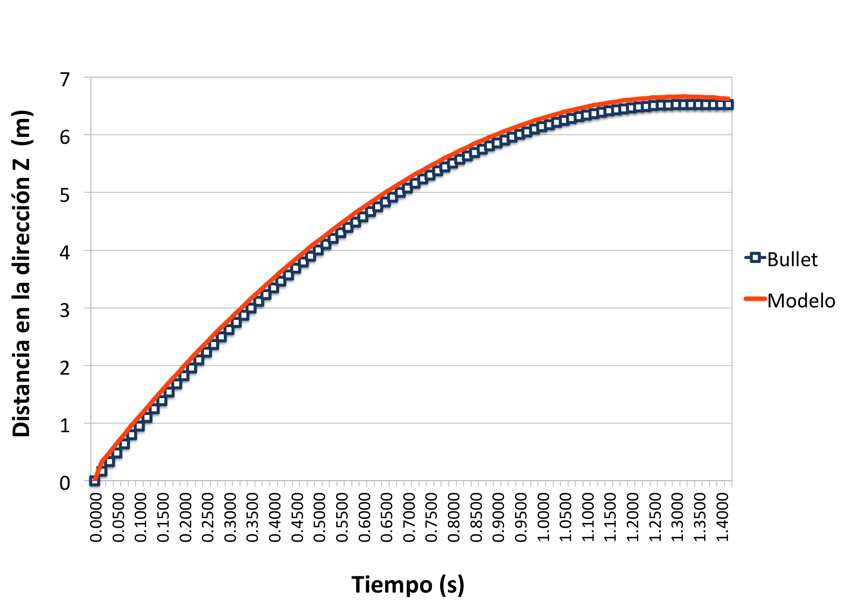
\includegraphics[width=0.6\linewidth]{image002.png} 
	\label{fig1:a} 
  }%
  \\
  \subfloat[][]{
  	\centering
	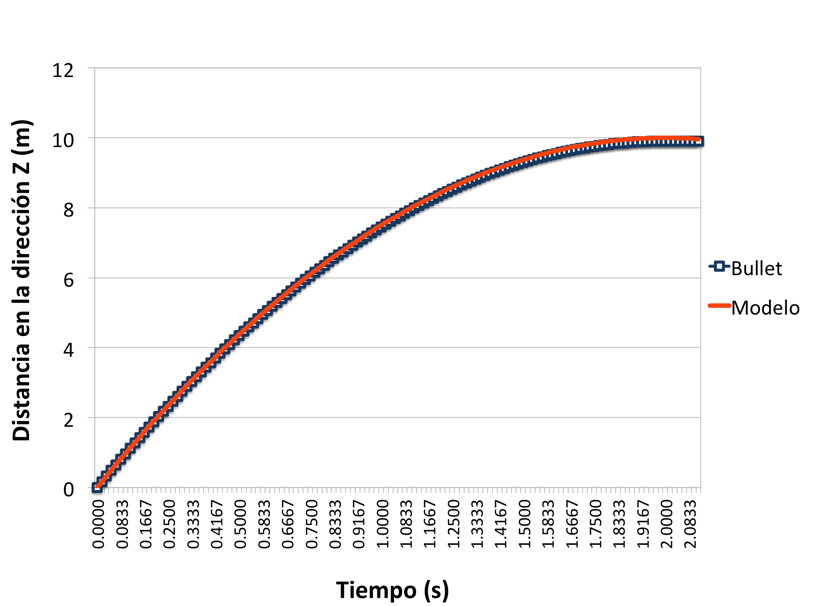
\includegraphics[width=0.6\linewidth]{image003.png} 
	\label{fig1:b} 
  }
  \\
  \subfloat[][]{
  	\centering
	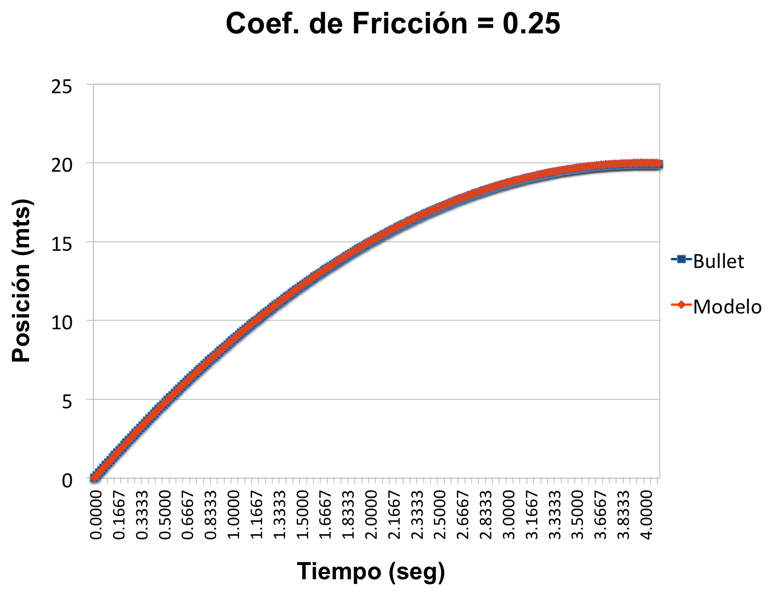
\includegraphics[width=0.6\linewidth]{image001.png} 
	\label{fig1:c} 
  }
  \caption{$v_i = 10 \frac{m}{s}$: (\protect\subref*{fig1:a}) $\mu_d=$0.25, (\protect\subref*{fig1:b}) $\mu_d=$0.50, y (\protect\subref*{fig1:c}) $\mu_d=$0.75}%
  \label{fig1} %
\end{figure}

\begin{figure}[H]%
  \centering
  \subfloat[][]{
  	\centering
	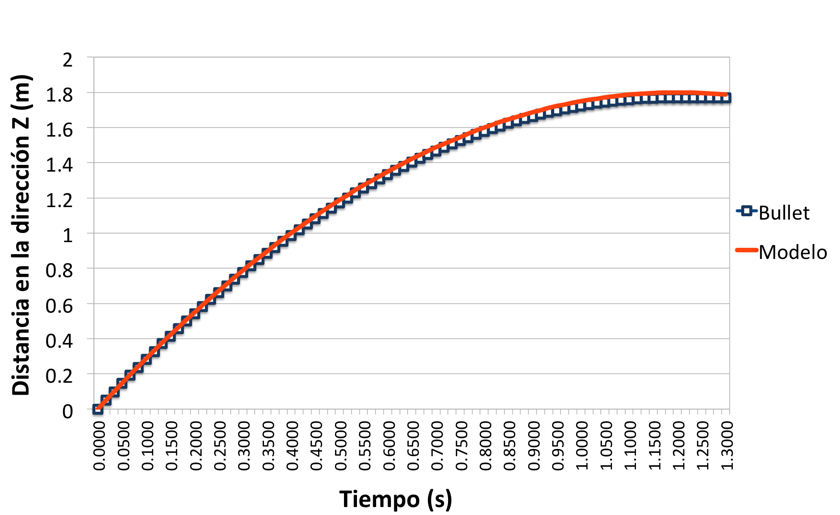
\includegraphics[width=0.6\linewidth]{image009.png} 
	\label{fig2:a} 
  }%
  \\
  \subfloat[][]{
  	\centering
	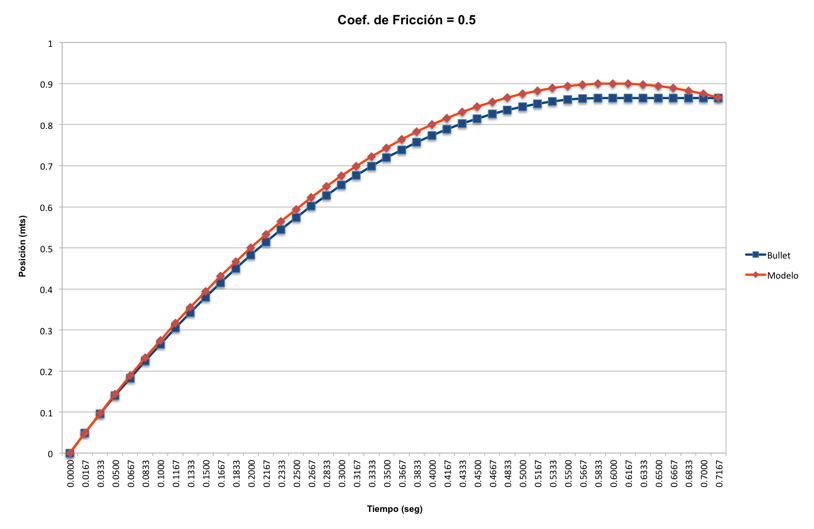
\includegraphics[width=0.6\linewidth]{image007.png} 
	\label{fig2:b} 
  }
  \\
  \subfloat[][]{
  	\centering
	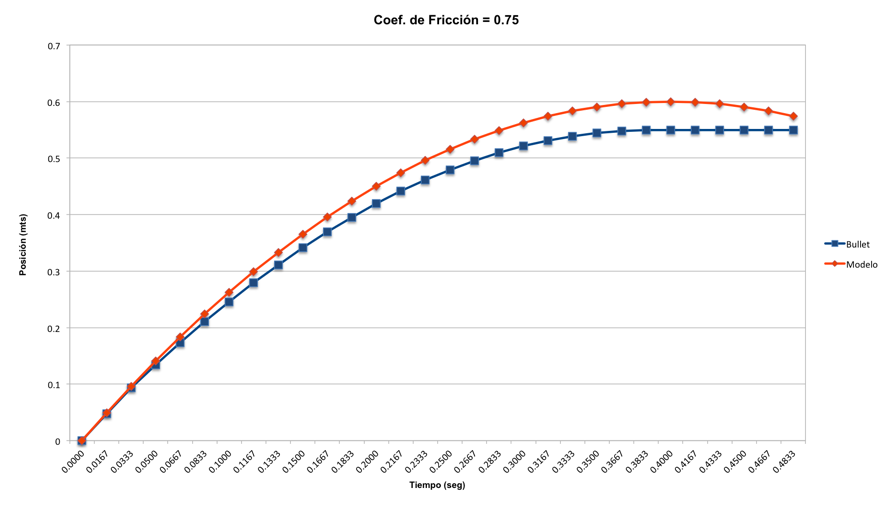
\includegraphics[width=0.6\linewidth]{image008.png} 
	\label{fig2:c} 
  }
  \caption{$v_i = 3 \frac{m}{s}$: (\protect\subref*{fig2:a}) $\mu_d=$0.25, (\protect\subref*{fig2:b}) $\mu_d=$0.50, y (\protect\subref*{fig2:c}) $\mu_d=$0.75}%
  \label{fig2} %
\end{figure}

\begin{figure}[H]%
  \centering
  \subfloat[][]{
  	\centering
	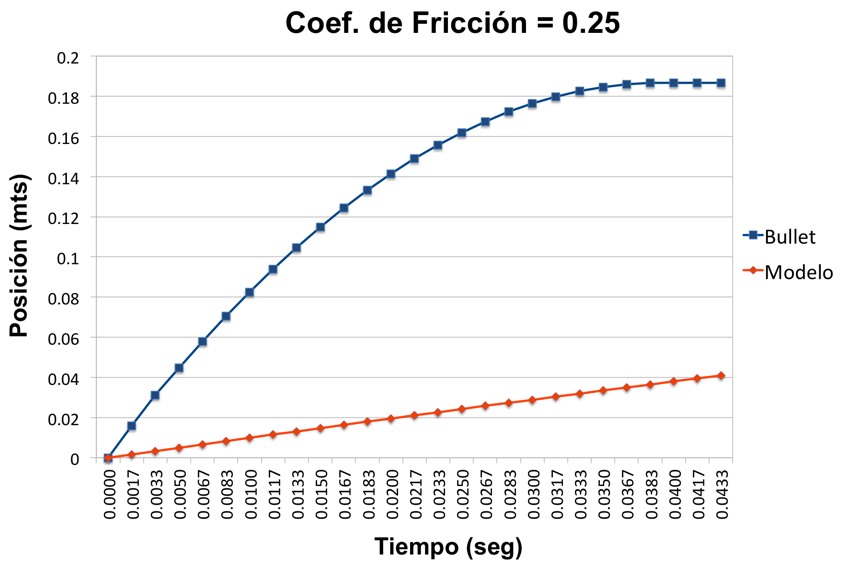
\includegraphics[width=0.6\linewidth]{image004.png} 
	\label{fig3:a} 
  }%
  \\
  \subfloat[][]{
  	\centering
	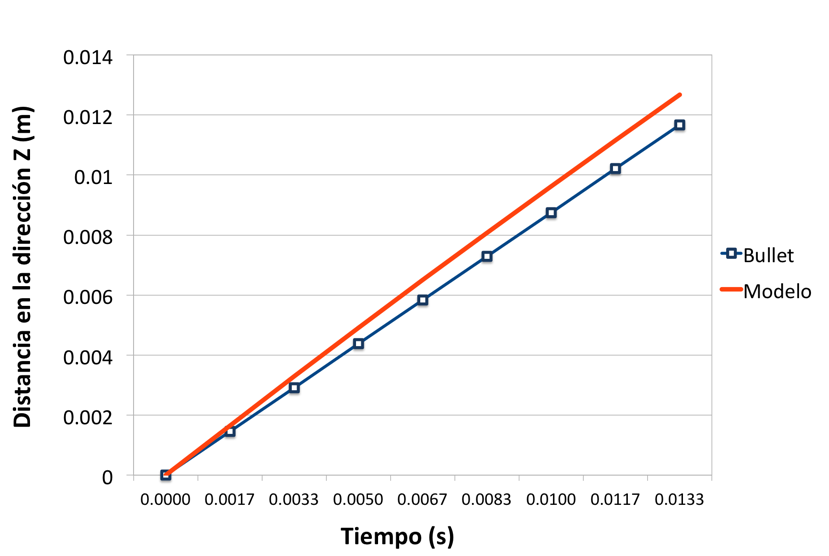
\includegraphics[width=0.6\linewidth]{image005.png} 
	\label{fig3:b} 
  }
  \\
  \subfloat[][]{
  	\centering
	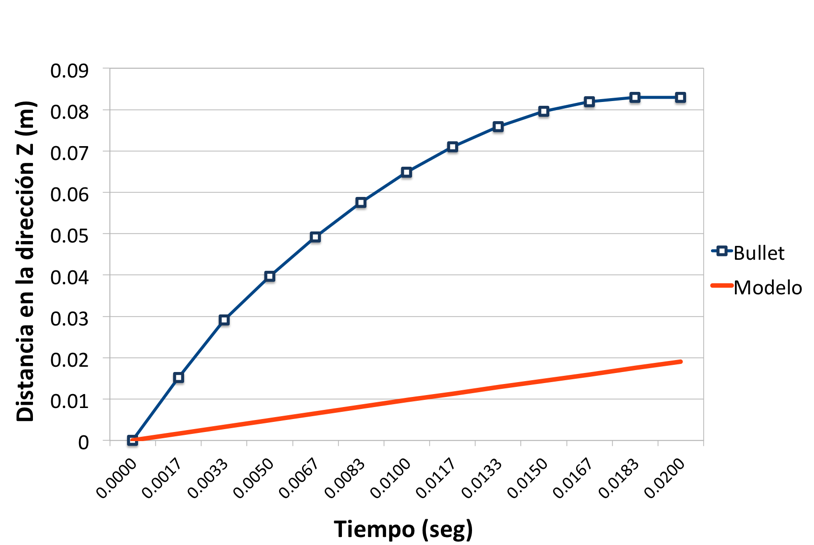
\includegraphics[width=0.6\linewidth]{image006.png} 
	\label{fig3:c} 
  }
  \caption{$v_i = 1 \frac{m}{s}$: (\protect\subref*{fig3:a}) $\mu_d=$0.25, (\protect\subref*{fig3:b}) $\mu_d=$0.50, y (\protect\subref*{fig3:c}) $\mu_d=$0.75}%
  \label{fig3} %
  \vspace*{6ex}
\end{figure}




\item El segundo simula una esfera a una altura determinada sobre el suelo, que tiene una velocidad en el eje perpendicular al piso y que eventualmente colisiona contra el mismo. \\
Se desea comprobar que la colisi\'on entre el cuerpo y el suelo respete que la velocidad final de la esfera despu\'es del choque sea proporcional a su coeficiente de restituci\'on $e$ dado por la ecuaci\'on:\\ 
 \begin{equation}
 \label{eq:restitution_coef}
  e = \frac{v_f}{v_i} 
\end{equation}
\\
Para efectuar la colisi\'on con el suelo, se emple\'o una esfera s\'olida ubicada a 4 metros del suelo, cuya masa y radio son $m_{sphere} = 1\ kg$ y $r_{sphere}=1\ m$,
respectivamente -ver Fig. \ref{fig:fallingBall}-. \\
En el ambiente utilizado no hay gravedad ($g = 0 \frac{m}{s}$), lo que posibilita utilizar la ecuaci\'on \eqref{eq:restitution_coef}.
El intervalo de tiempo f\'isico (o \textit{timestep}) utilizado es $\Delta t=0.001 s$). El \textit{timestep} de animaci\'on (es decir,
cada cu\'anto tiempo se guardan en un archivo los datos logrados) es $\Delta t' = 0.1$ y el tiempo de simulaci\'on es de $s=100\Delta t$. El coeficiente de fricci\'on es $\mu = 0.75$.\\

\begin{figure}[H]%
  \centering
  \frame{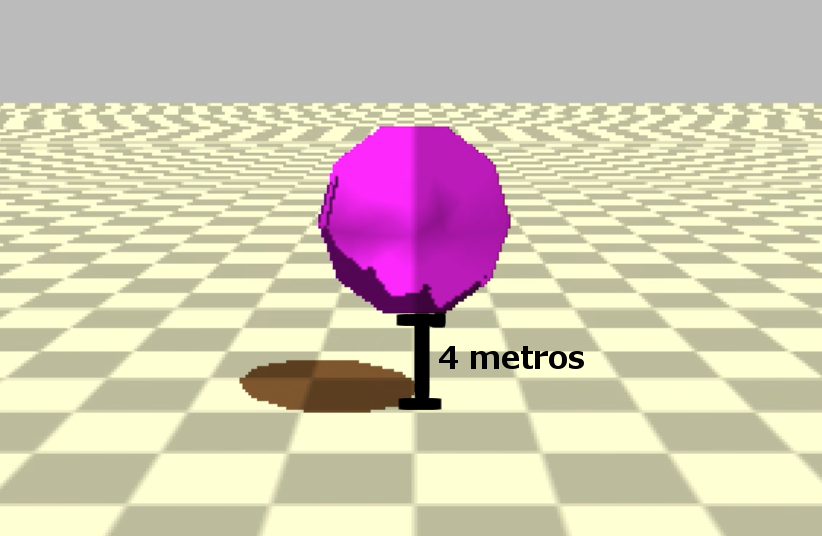
\includegraphics[width=0.4\linewidth]{fallingBall.png}}
    \caption{Esquema del segundo experimento}
    \label{fig:fallingBall} 
\end{figure} 

El experimento tiene como par\'ametros de entrada: $v_{i}$ (velocidad inicial) y $e_{sim}$ (coeficiente de restituci\'on esperado). Por otro lado, se obtiene $v_{f}$ (velocidad de la esfera al finalizar la simulaci\'on); y se calculan $e_{medida}$ (coeficiente de restituci\'on obtenido a partir de \eqref{eq:restitution_coef}) y $\epsilon_{rel}$ (error relativo entre los coeficientes $e_{sim}$ y $e_{medida}$).  \\
Acto seguido, se muestran los experimentos realizados. En ellos, $v_{i}= \{$ -0.5, -3.5 y -4$\} \frac{m}{s}$ y $e_{sim}= \{ $0.25, 0.5 y 0.8$\} $.\\

\begin{table}[H]%
  \centering
  \subfloat[][]{
  	\label{table1a}
  	\begin{tabular}{ | c || c | c | c | }
	  		\hline
	  		$e_{sim}$ & 0.2 & 0.5 &  0.8 \\
			\hline 
	  		$v_{f}$ & 0.000249  $\frac{m}{s}$& 0.000219  $\frac{m}{s}$& 0.001037  $\frac{m}{s}$\\
	  		\hline
	  		$e_{medida}$ & 0.000498 & 0.000438 & 0.002074 \\
	  		\hline
	  		$\epsilon_{rel}$ & 0.997 & 0.999 & 0.997 \\
	  		\hline
	\end{tabular}
  }%
  \qquad
  \subfloat[][]{
  	\label{table1b}
  	\begin{tabular}{ | c || c | c | c | }
	  		\hline
	  		$e_{sim}$ & 0.2 & 0.5 &  0.8 \\
			\hline 
	  		$v_{f}$ & 0.000057  $\frac{m}{s}$ & 0.000018  $\frac{m}{s}$ & 0.3  $\frac{m}{s}$\\
	  		\hline
	  		$e_{medida}$ & 0 & 0 & 0.0857 \\
	  		\hline
	  		$\epsilon_{rel}$ & 1 & 1 & 0.893 \\
	  		\hline
	\end{tabular}
  
  }
  \qquad
  \subfloat[][]{
  	\label{table1c}
  	\begin{tabular}{ | c || c | c | c | }
	  		\hline
	  		$e_{sim}$ & 0.2 & 0.5 & 0.8 \\
			\hline 
	  		$v_{f}$ & 0.000473  $\frac{m}{s}$ & 0.000424   $\frac{m}{s}$& 1.23  $\frac{m}{s}$\\
	  		\hline
	  		$e_{medida}$ & 0.00012 & 0.00011 & 0.3 \\
	  		\hline
	  		$\epsilon_{rel}$ & 1 & 1 & 0.625 \\
	  		\hline
	\end{tabular}
  }
  \\
  \subfloat[][]{
	\label{table1d}
  	\begin{tabular}{ | c || c | c | c | }
	  		\hline
	  		$e_{sim}$ & 0.2 & 0.5 & 0.8 \\
			\hline 
	  		$v_{f}$ & 1  $\frac{m}{s}$& 2.5  $\frac{m}{s}$& 4  $\frac{m}{s}$\\
	  		\hline
	  		$e_{medida}$ & 0.2 & 0.5 & 0.8 \\
	  		\hline
	  		$\epsilon_{rel}$ & 0 & 0 & 0 \\
	  		\hline
	\end{tabular}
  }
  \qquad
  \subfloat[][]{
  	\label{table1e}
  	\begin{tabular}{ | c || c | c | c | }
	  		\hline
	  		$e_{sim}$ & 0.2 & 0.5 & 0.8 \\
			\hline 
	  		$v_{f}$ & 2  $\frac{m}{s}$& 5  $\frac{m}{s}$& 8  $\frac{m}{s}$\\
	  		\hline
	  		$e_{medida}$ & 0.2 & 0.5 & 0.8 \\
	  		\hline
	  		$\epsilon_{rel}$ & 0 & 0 & 0 \\
	  		\hline
	\end{tabular}
  }
  \caption{Coeficientes de restituci\'on obtenidos de simular el sistema descripto en Fig. \ref{fig:fallingBall}:  \\ (\protect\subref*{table1a}) $v_i = -0.5 \frac{m}{s}$, (\protect\subref*{table1b}) $v_i = -3.5 \frac{m}{s}$, (\protect\subref*{table1c}) $v_i = -4 \frac{m}{s}$, (\protect\subref*{table1d}) $v_i = -5 \frac{m}{s}$, y (\protect\subref*{table1e}) $v_i = -10 \frac{m}{s}$ }%
  \label{table1}%
\end{table}

Los resultados exponen una limitaci\'on del motor f\'isico: no representa correctamente las colisiones el\'asticas entre esferas y cuerpos r\'igidos, que ocurren a velocidades bajas. Esto queda en evidencia en la Tabla \ref{table1}. En cada una de ellas el error fue de casi el 100\%.\\
La raz\'on por la que ocurre este hecho se debe a que \textit{Bullet} utiliza un algoritmo de colisi\'on que frena la velocidad de un objeto que est\'a a punto de colisionar. Haciendo esto puede evitar que los s\'olidos se traspasen y de esta forma se pueden realizar c\'alculos de fuerza m\'as precisos. En el caso de los experimentos, las esferas poseen una rapidez muy baja, cuando est\'an a punto de colisionar \textit{Bullet} reduce a\'un m\'as esta velocidad y eventualmente quedan con una velocidad tan baja que al chocar contra el suelo se aplica el efecto restitutivo a esta velocidad casi nula y se resuelve que la esfera debe quedar en reposo, cuando en realidad deber\'ia poseer una velocidad baja, pero no despreciable. \\

\end{itemize}


%\end{adjustwidth}

\subsubsection{Ventajas}
%\begin{adjustwidth}{1.3cm}{0cm}
\begin{itemize}[leftmargin=5.5mm]
\item C\'odigo abierto: mayor conocimiento sobre las f\'ormulas y m\'etodos implementados en el motor, a diferencia de lo acaecido en trabajos previos \cite{Cuadrupedo}, en donde al usar frameworks f\'isicos de c\'odigo cerrado, no se ten\'ia ni control ni conocimiento pleno de su funcionamiento.
\item Soporte de la comunidad cientf\'ifica.
\item Licencia libre.
\\
\end{itemize}
%\end{adjustwidth}

\subsubsection{Desventajas}
%\begin{adjustwidth}{1.3cm}{0cm}
\begin{itemize}[leftmargin=5.5mm]
\item Documentaci\'on poco clara y desordenada.
\item Debido a que la f\'isica se aproxima usando m\'etodos num\'ericos que contienen error, las simulaciones son no determin\'isticas.
\item Utilizar una librer\'ia gr\'afica (como \textit{OpenGL}) acoplada a una simulaci\'on  de \textit{Bullet} puede producir resultados distintos que si se utiliza un programa de visualizaci\'on externo (como OVITO).
\\
\end{itemize}
%\end{adjustwidth}




\subsection{Librer\'ia de Algoritmos Gen\'eticos}

%\begin{adjustwidth}{1.2cm}{0cm}
Se utiliz\'o la conocida librer\'ia de Algoritmos Gen\'eticos para C++ GaLib, desarrollada por Matthew Wall del MIT \cite{LinkGaLib}. \\
Ofrece funcionalidades como: programaci\'on paralela, diversos m\'etodos de selecci\'on (elite, ruleta), estrategias de reemplazo (de padres, aleatorio, del peor), entre otras.\\

%\end{adjustwidth}

\subsection{C\'odigo Fuente}

%\begin{adjustwidth}{1.2cm}{0cm}
Al estar \textit{Bullet} implementado en C++, el c\'odigo fuente tambi\'en est\'a desarrollado en ese lenguaje. En \textit{Bullet}, se define un \textit{World} -o mundo f\'isico- en donde se puede insertar, entre otras cosas, cuerpos r\'igidos. En este caso en particular, el mundo consta de un plano  -el suelo- y  el humanoide encima -compuesto por cuerpos r\'igidos y otros elementos f\'isicos-. \\
El software creado incluye: creaci\'on del humanoide, siendo \'este capaz de desplazarse por medio de actuadores (que se ver\'an en la Secci\'on \ref{actuadores}); el desarrollo del algoritmo gen\'etico (la definici\'on de los individuos, la funci\'on de fitness, m\'etodos de selecci\'on, etc.); visualizaci\'on gr\'afica del mejor humanoide logrado por el algoritmo gen\'etico; y la posibilidad de realizar gr\'aficos referidos a la evoluci\'on del algoritmo gen\'etico (fitness por cada generaci\'on, etc.). \\
Se acompa\~nan a esta presentaci\'on: el c\'odigo fuente y el manual de instalaci\'on y uso.

%\end{adjustwidth}

%\end{adjustwidth}



\section{Modelo Utilizado}

%\begin{adjustwidth}{1.1cm}{0cm}
Hay diversos modelos. Algunos son m\'as gen\'ericos \cite{flexibleMuscle} \cite{Wojtyra} y complejos.  Sin embargo, se procur\'o utilizar uno que fuera sencillo pero representativo a la vez.\\ 
Se modela al cuerpo humano, con el motor \textit{Bullet Physics}, como un conjunto de segmentos unidos por articulaciones. A cada uno de ellos se les aplica una fuerza en el centro de masa de cada segmento (denominada Actuador). Que la caminata se produzca o no, depende del tipo de actuador utilizado (la funci\'on utilizada para la fuerza), y de sus par\'ametros. El objetivo, entonces, se reduce a encontrar dichos par\'ametros. Para eso se usan los algoritmos gen\'eticos, un m\'etodo de Inteligencia Artificial. De este modo, se obtiene, de forma an\'aloga a la selecci\'on natural, los individuos que mejor se adapten a la caminata. Tanto los actuadores como el algoritmo gen\'etico se explicar\'an m\'as adelante. \\ 

\begin{figure}[H]%
  \centering
  \frame{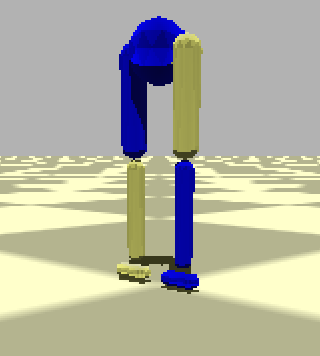
\includegraphics[width=0.3\linewidth]{humanoid.png}}  
    \caption{Humanoide dise\~nado}
    \label{fig:humanoid}
\end{figure} 

\subsection{Composici\'on F\'isica del Humanoide}
\textbf{No est\'a terminada a\'un} \\
Como ya se dijo, el humanoide fue modelado en \textit{Bullet} como un conjunto de segmentos, unidos por articulaciones. Los segmentos son cuerpos rig\'idos 

Se dividi\'o al cuerpo humano en los siguientes segmentos: cabeza, tronco, miembro superior, pelvis y miembro inferior (muslo, pierna y pie). Considerar la mitad superior del cuerpo implicaba tener -ver Fig. \ref{fig:seg_and_art}-.    \\ \\
A continuaci\'on se presenta la composici\'on de cada segmento (de acuerdo a la biomec\'anica \cite{biomechanics}): 
\begin {table}[ht]
	\begin{center}
		\begin{tabular}{ | c | c | c | c | c | c |}
	  		 \hline
	  		Parte & Cantidad & Forma & Largo (en m) & Peso (en kg) & Uniones\\
	  		\hline 
	  		\hline
	  		Pelvis & 1 & esf\'erico & 0.08655 & 9.9718 & Cadera\\
	  		\hline
	  		Muslo & 2 & esfero-cilindro & 0.4015 & 10.3368 & Cadera y Rodilla\\
	  		\hline
	  		Pierna & 2 & esfero-cilindro &  0.4015 & 3.1609 & Rodilla y Tobillo\\
	  		\hline
	  		Pie & 2 & esfero-cilindro & - & 1.0001 & Tobillo\\
	  		\hline
		\end{tabular}
		\caption{Segmentos del humanoide}
	\end{center}
\end{table}

\begin{figure}[H]%
  \centering
  \subfloat[][]{
  	\centering
	  \frame{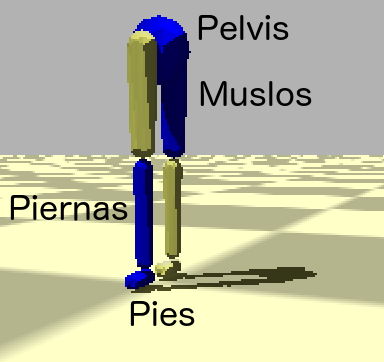
\includegraphics[width=0.35\linewidth]{humanoid_segments.png}} 
	\label{fig7:a} 
  }
  \qquad
  \subfloat[][]{
  	\centering
	  \frame{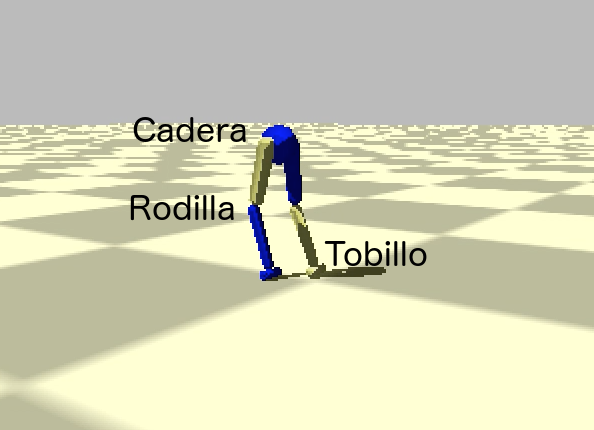
\includegraphics[width=0.45\linewidth]{humanoid_articulations.png}}
	\label{fig7:b} 
  }
  \caption{Humanoide dise\~nado: (\protect\subref*{fig7:a}) segmentos, y (\protect\subref*{fig7:b}) articulaciones}%
  \label{fig:seg_and_art} %
\end{figure}


%\end{adjustwidth}

\subsection{Articulaciones}
\textbf{No est\'a terminada a\'un} \\
Para unir los distintos segmentos entre s\'i, se utilizaron articulaciones bisagra con 1 grados de libertad: en el eje Z -en donde ocurre la caminata- y en el eje Y -el perpendicular al piso-. Adem\'as, para cada caso en particular, se definieron cotas para los \'angulos que pueden existir entre los segmentos. Esto es muy importante, no s\'olo porque se adec\'ua a datos biol\'ogicos, sino porque, de otro modo la caminata no podr\'ia lograrse: si los \'angulos son demasiado altos, la caminata se produce girando las piernas por encima de la pelvis; si por el contrario, son demasiado bajos, las piernas van a estar muy r\'igidas, originando pocos pasos y muy cortos. 
Tanto para la  \\
Por otra parte, a la pelvis se le restringe todo tipo de rotaci\'on. 

\section{Actuadores}
\label{actuadores}
%\begin{adjustwidth}{1.1cm}{0cm}
A cada uno de los segmentos correspondientes al muslo y la pierna del b\'ipedo, se le aplica un torque -o actuador- en el eje X -perpendicular a la trayectoria-, como se ve en Fig \ref{fig:actuator}. As\'i, pueden moverse para arriba o para abajo -con respecto a la articulaci\'on a la que pertenecen-. A fin de simplificar el modelo, el humanoide tiene el mismo tipo de actuador utilizado en todos los segmentos.\\
Que el torque se aplique en una sola dimensi\'on, contribuye a que la caminata producida sea plana -en 2D, y no en 3D, como deber\'ia ser en una caminata real-.\\ 
Para indicar el m\'odulo de dicho torque, se dise\~naron diferentes funciones (todas ellas peri\'odicas), mencionadas en las siguientes subsecciones. \\
\begin{figure}[H]%
  \centering
  \frame{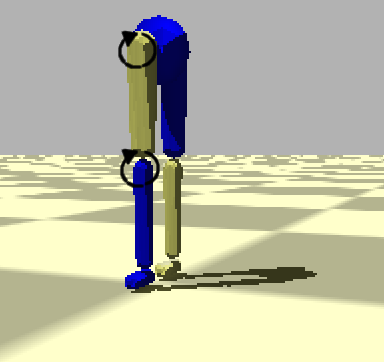
\includegraphics[width=0.4\linewidth]{actuators.png}}
    \caption{Aplicaci\'on de los actuadores en los segmentos del b\'ipedo}
    \label{fig:actuator} 
\end{figure} 

\subsection{Gen\'erico}
Es el actuador m\'as sencillo (tanto matem\'atica como computacionalmente). No se consideraron las funciones trigonom\'etricas b\'asicas (es decir, solo $\sin$ o $\cos$), por los resultados obtenidos en \cite{Cuadrupedo}. La fase es la misma tanto en el seno como en el coseno, para evitar que se formen otro tipo de funciones no c\'iclicas ($f(t)=0$).
\begin{equation}
  f(t) =  A_1 \sin(\omega_1t+\phi)+A_2 \cos(\omega_2t+\phi)+C
\end{equation}

\subsection{Fourier}
Este actuador utiliza una serie de Fourier de dos t\'erminos. 
\begin{equation}
  f(t) =  A_1 \sin(\omega t+\phi)+B_1 \cos(\omega t+\phi)+A_2 \sin(2\omega t+\phi)+B_2 \cos(2\omega t+\phi)+C
\end{equation}

\subsection{Extra Fourier}
Es una extensi\'on del actuador anterior, pero con 9 t\'erminos. Por ser de mayor grado, brinda una mayor precisi\'on. Sin embargo, es m\'as dificil de manejar computacionalmente; y, adem\'as, que sea m\'as preciso no garantiza que con \'el se pueda lograr una buena caminata.
\begin{equation}
\begin{split}
  f(t) = &   A_1 \sin(\omega t+\phi)+B_1 \cos(\omega t+\phi)+A_2 \sin(2\omega t+\phi)+B_2 \cos(2\omega t+\phi) \\
  &+A_3 \sin(3\omega t+\phi)+B_3 \cos(3\omega t+\phi)+A_4 \sin(4\omega t+\phi)+B_4 \cos(4\omega t+\phi) \\ 
  &+A_5 \sin(5\omega t+\phi)+B_5 \cos(5\omega t+\phi)+A_6 \sin(6\omega t+\phi)+B_6 \cos(6\omega t+\phi) \\
  &+A_7 \sin(7\omega t+\phi)+B_7 \cos(7\omega t+\phi)+A_8 \sin(8\omega t+\phi)+B_8 \cos(8\omega t+\phi) \\
  &+A_9 \sin(9\omega t+\phi)+B_9 \cos(9\omega t+\phi) + C
\end{split}
\end{equation}

\subsection{Doble coseno}
Esta funci\'on peri\'odica utiliza medio ciclo de una funci\'on sinusoidal, y medio ciclo de otra (ambas pueden tener frecuencias distintas). De esta manera, se consigue una caminata m\'as natural, y que no ocurre con los actuadores de Fourier, que producen una doble flexi\'on de las rodillas en cada ciclo.\\
La idea es lograr una funci\'on peri\'odica a partir de una que no lo es (ya que $t$ es lineal). Para eso, se utiliza $\psi (t)$ -ec. \eqref{eq:phi}- que aplica una transformaci\'on a los n\'umeros reales, para que se encuentren dentro del rango del ciclo completo (con las dos frecuencias). $\omega$ es la frecuencia de $f(t)$ -ec. \eqref{eq:ft}-, que utiliza medio ciclo con frecuencia $\omega_1$ y medio ciclo con frecuencia $\omega_2$.
\begin{equation} 
\label{eq:phi}
\begin{aligned}[c]
\psi (t) = t+ \phi- \floor[\Bigg]{ \frac{t+\phi}{\pi/\omega_1+\pi/\omega_2} } (\pi/\omega_1+\pi/\omega_2) 
 \end{aligned}
 \qquad
 \begin{aligned}[c]
 \psi: \mathbb{Re} \rightarrow \bigg[0, \frac{2\pi}{\omega}\bigg] 
 \end{aligned}
\end{equation}
 \\
\begin{equation}
\omega = \frac{2\omega_1 \omega_2}{\omega_1+\omega_2} 
 \end{equation}
\\
\begin{equation}
\label{eq:ft}
f(t) =  \left\{
\begin{array}{ll}
      A \cos(\omega_1 \psi(t))+C & \mbox{si $\omega_1 \psi(t) < \pi$}  \\
      A \cos(\omega_2 (\psi(t) - (\pi/\omega_1) + (\pi/\omega_2 ) ) )+C & \mbox{en otro caso$$} \\
\end{array} 
\right. 
 \end{equation}

\section{Condiciones iniciales y de contorno}
Las funciones peri\'odicas mencionadas en los actuadores no son suficientes para lograr la caminata. 
A los actuadores mencionados previamente, se le adosaron las funciones vistas a continuaci\'on. 
\subsection{Funci\'on Partida}
El andar del humanoide es c\'iclico. Sin embargo, por la posici\'on inicial del individuo, se requiere para el tiempo del primer paso, una funci\'on distinta a la del resto de la caminata. El tipo de funci\'on puede ser cualquiera de los actuadores vistos anteriormente (pero no necesariamente con los mismos valores de amplitud, frecuencia y fase asignados a las piernas). Empero, se utiliz\'o la funci\'on vista en el actuador gen\'erico. \\
Por otra parte, para simplificar el modelo, se decidi\'o  que el tiempo considerado para el primer paso sea fijo, y de 0.7 segundos. Dicho valor fue extra\'ido de forma experimental.

\subsection{Fase sincronizada}
En una caminata, las piernas deben guardar simetr\'ia: mientras una va hacia adelante, la otra va hacia atr\'as (y viceversa). Esto, de acuerdo con  los actuadores definidos en la secci\'on anterior, implica que las funciones de movimiento de cada pierna est\'en desfasadas en medio ciclo ($\frac{\pi}{2}$):
\begin{equation}
f_{izquierda}(t) =  f(t)
 \end{equation}
 \begin{equation}
f_{derecha}(t) =  f(t+\frac{\pi}{2})
 \end{equation}
siendo $f(t)$ la funci\'on de movimiento (o actuador) en el momento $t$.
%\begin{adjustwidth}{1.1cm}{0cm}

%\end{adjustwidth}


%----------------------------------------------------------------------------------------
%	SECTION 2
%----------------------------------------------------------------------------------------

\section{Algoritmo Gen\'etico}


\subsection{Individuo}

%\begin{adjustwidth}{1.25cm}{0cm}
Es por eso que el individuo, en este caso, est\'a compuesto por un array de n\'umeros, que identifican tanto los valores asociados a las fuerzas de los actuadores. 
%\end{adjustwidth}

\subsection{Fitness}

%\begin{adjustwidth}{1.25cm}{0cm}
El papel de la funci\'on de fitness $F$ en un algoritmo gen\'etico es evaluar qu\'e tan bueno es un individuo. En este caso, est\'a definida como un producto de cinco m\'odulos o propiedades: altura ($H$), velocidad ($V$), direcci\'on ($D$), simetr\'ia ($S$) y pies abajo ($PA$):
\begin{equation}
  F = H * V *D * S *  PA
\end{equation}
Los cuatro tienen la misma importancia y, por eso, como se ver\'a a continuaci\'on, est\'an definidos de forma similar (con una funci\'on exponencial y pueden valer entre 0 y 1). Con todo esto, dado que el fitness est\'a pensado como un producto, basta con que uno de los m\'odulos sea muy chico para  ``anular'' al individuo -es decir, otorgarle un valor que tiende a cero-. Sin embargo, los diferentes m\'odulos no son completamente independientes entre s\'i: por ejemplo, si la altura es demasiado baja, posiblemente la velocidad y la direcci\'on no sean adecuadas. \\
%\end{adjustwidth}

\subsubsection{Altura}
\label{altura}
%\begin{adjustwidth}{1.4cm}{0cm}
Es un factor relacionado con la altura del individuo en toda la simulaci\'on, y se expresa:\\
\begin{equation}
  H = \frac{\sum_{n=0}^{T} {e^{-C( h_{t_{n}} - h_{t_{0}} )^2  }}}{N}
\end{equation}
\\ donde $t_{0}$ es el tiempo inicial, $t_{T}$ el tiempo final, $N$ la cantidad pasos de simulaci\'on y $C$ una constante $C=5$.
\\
Se calcula a partir de la diferencia entre la altura en cada instante de la simulaci\'on, con su altura inicial -la altura est\'a definida como la posici\'on de la pelvis en el eje Z-. Cuanto mayor sea esa diferencia, m\'as r\'apido el individuo cae, y por eso este m\'odulo tiende a cero. Por el contrario, valdr\'a uno si la diferencia es \'infima -lo que significa que el humanoide mantiene su misma altura durante la caminata-.\\

%\end{adjustwidth}

\subsubsection{Velocidad}
\label{velocidad}
%\begin{adjustwidth}{1.4cm}{0cm}
Indica qu\'e tan cercana es la velocidad del individuo con respecto a una velocidad objetivo -en este caso, es de 1.2 m/h-, y se expresa de la siguiente forma:\\
\begin{equation}
  V = \frac{\sum_{n=0}^{T} {e^{-C( \|v_{t_{n}}\| - V_{O} )^2  }}}{N}
\end{equation}
\\ donde $t_{0}$ es el tiempo inicial, $t_{T}$ el tiempo final y $V_{O}$ la velocidad objetivo en el eje Z -el eje de la caminata-.
\\
Sigue una l\'ogica y c\'alculo similares al factor de altura: a mayor discrepancia de la velocidad real del humanoide con $V_{O}$, menor -y m\'as cercano a cero- es el valor arrojado por el m\'odulo de velocidad. 

%\end{adjustwidth}

\subsubsection{Direcci\'on}
\label{direccion}
%\begin{adjustwidth}{1.4cm}{0cm}
Se\~nala qu\'e tan similares son la direcci\'on objetivo -un vector unitario, que en este caso se encuentra en el eje Z- y la direcci\'on con la que camine el humanoide. Se calcula como sigue:\\
\begin{equation}
 D = \frac{\sum_{n=0}^{T} {e^{-C( \vec{v_{t_{n}}} \cdot \vec{V_{O} } -1)^2 } } }{N}
\end{equation}
\\ donde $t_{0}$ es el tiempo inicial, $t_{T}$ el tiempo final, $\vec{v_{t_{n}}}$ el versor de la direcci\'on del humanoide en el momento $t_{n}$ y $\vec{V_{O}}$ el versor de la direcci\'on objetivo.
\\ El producto escalar entre los versores responde a la Similitud Coseno: $\cos \theta = \frac{A \cdot B} {\|A\|\|B\| } $, donde A y B son vectores que no se encuentran normalizados, y $\theta$ es el \'angulo formado entre ellos. As\'i,  si $\cos \theta=1$, significa que los vectores est\'an paralelos entre s\'i -que es el efecto buscado en el caso de la direcci\'on-. 
\\ Al producto escalar se le resta 1, para que el m\'odulo sea consistente con la funci\'on exponencial utilizada y que valga 1 cuando $\theta = 0$, y  0 cuando $\theta = \pi$. Cabe aclarar que se trata al \'angulo en forma sim\'etrica, ya que, por ejemplo $\cos(-\pi/6) = \cos(\pi/6)$.\\

\subsubsection{Simetr\'ia}
\label{simetria}
Se\~nala qu\'e tan equidistantes se encuentran los pies de la cadera, a lo largo de la caminata. Aplicando solamente los m\'odulos antes mencionados, provocaba resultados en donde una pierna quedaba m\'as distante de la pelvis que la otra, lo que provocaba que el humanoide se terminara arrastrando (y posiblemente afectando a la velocidad).\\
Para mayor simplicidad, la simetr\'ia $S$ se calcul\'o a partir de los pies (y no de las piernas). Se tomaron en cuenta s\'olo los ejes X y Z, porque son los relacionados a la velocidad y a la direcci\'on, respectivamente.
\begin{equation}
 S = \frac{\sum_{n=0}^{T} { \frac{1}{2} [e^{-C( lf_{Z} + rf_{Z}| ^2) } + e^{-C( lf_{X} + rf_{X}| ^2) }]  } } {N}
\end{equation}
\\ donde $lf_{X} $ y $lf_{Z} $ es la distancia desde el pie izquierdo hasta la pelvis en los ejes X y Z, respectivamente; y  en donde $rf_{X} $ y $rf_{Z} $ es lo mismo, pero para el pie derecho. \\

\subsubsection{Pies abajo}
\label{piesabajo}
Con los m\'odulos se�alados anteriormente, se resalta que el humanoide camine con una velocidad y direcci\'on determinadas, que no se caiga y que mantenga simetr\'ia mientras ejecuta sus movimientos. Pero, todo esto dar\'ia, en el mejor de los casos, una caminata estilo ``estrella". \\
Sin embargo, una caracter\'istica fundamental en una caminata normal es que las piernas (ergo, los pies tambi\'en) no sobrepasen la cadera. Si bien \'esta es una propiedad negativa (expresa lo que no debe tener una caminata), y se puede correr el riesgo de restringir demasiado, su ausencia da resultados peores.
\begin{equation}
 PA = \frac{\sum_{n=0}^{T} { \frac{1}{2} ( \alpha  [e^{-C( ldf ^2) } + e^{-C( rdf ^2) }]  } } {N}
\end{equation}
\\ donde  $\alpha = max(min(lf,rf)-hip,0),1) $ (es decir, vale 0 si la altura del pie izquierdo o derecho supera a la de la cadera, y 1 en otro caso); y $ldf $ y $rdf $ es la diferencia entre la posici\'on inicial de los pies y la altura en el momento $t_{n}$ de los pies izquierdo y derecho, respectivamente. \\
%\end{adjustwidth}



%----------------------------------------------------------------------------------------
%	SECTION 3
%----------------------------------------------------------------------------------------

\subsection{Par\'ametros del Algoritmo}

\subsubsection{M\'etodos de selecci\'on}
\label{metodos de seleccion}
%\begin{adjustwidth}{1.4cm}{0cm}
De la vasta cantidad de m\'etodos de selecci\'on que existen, se utilizaron: \textbf{\textit{Elite}} -en donde se selecciona el individuo con mayor aptitud de la poblaci\'on-; y \textbf{\textit{Roulette}} -m\'etodo probabil\'istico, que selecciona un individuo de la poblaci\'on total al azar, con una probabilidad proporcional a su \textit{fitness}-.
%\end{adjustwidth}

\subsubsection{M\'etodos de cruza}
\label{metodos de cruza}
%\begin{adjustwidth}{1.4cm}{0cm}
El m\'etodo de cruza -o \textit{crossover}- utilizado es el siguiente: De dos individuos -los padres-, se originan dos nuevos individuos -los hijos-. Se toma cada uno de los genes de los padres y se elige, con una probabilidad uniforme, uno de ellos para un hijo y el otro para el otro hijo.\\
La probabilidad de que este proceso ocurra es de 0.9.

%\end{adjustwidth}

\subsubsection{Mutaci\'on}
\label{mutacion}
%\begin{adjustwidth}{1.4cm}{0cm}
En el caso de la mutaci\'on, se selecciona cada gen del individuo, y se elige aleatoriamente -como una moneda- los bits que se modifican y los que no.\\
La probabilidad de que ocurra una mutaci\'on es de 0.3.
%\end{adjustwidth}



%----------------------------------------------------------------------------------------
%	SECTION 4
%----------------------------------------------------------------------------------------

\section{Resultados Obtenidos}
%\begin{adjustwidth}{1.1cm}{0cm}
cccccccvvvvv

\begin{figure}[h]
\begin{center}

\includegraphics[width=0.65\textwidth]{placeholder} % Include the image placeholder.png
\caption{Figure caption.}
\end{center}
\end{figure}
%\end{adjustwidth}

%----------------------------------------------------------------------------------------
%	SECTION 5
%----------------------------------------------------------------------------------------

\section{Conclusiones}

%\begin{adjustwidth}{1.1cm}{0cm}
xxxxxxxx
%\end{adjustwidth}

%----------------------------------------------------------------------------------------
%	BIBLIOGRAPHY
%----------------------------------------------------------------------------------------

\begin{thebibliography}{1}
\bibitem{wikiPhysicsEngine} Wikipedia: $https://es.wikipedia.org/wiki/Physics\_engine$
\bibitem{Comparissons}
Andreas Gerndt y otros, \emph{An Evaluation of Open Source Physics Engines for Use in Virtual Reality Assembly Simulations, Fecha de publicaci\'on: 2012}
\bibitem{Comparissons2}
Tom Erez y otros, \emph{Simulation Tools for Model-Based Robotics: Comparison of \textit{Bullet}, Havok, MuJoCo, ODE and PhysX}
\bibitem{LinkBullet} Sitio web de Bullet Physics: $http://www.bulletphysics.org/$
\bibitem{Catto}
Erin Catto, \emph{Iterative Dynamic with Temporal Coherence, Fecha de publicaci\'on: 2005}
\bibitem{Cuadrupedo}
Kevin Kenny, M\'aximo Videla y Axel Wassington, \emph{Proyecto Final para la obtenci\'on del t\'itulo: Ingeniero en Inform\'atica, 2014 - ITBA}
\bibitem{LinkGaLib} Sitio web de GaLib: $http://lancet.mit.edu/ga/$
\bibitem{flexibleMuscle}
Thomas Geijtenbeek, Michiel van de Panne y A. Frank van der Stappen, \emph{Flexible Muscle-Based Locomotion for Bipedal Creatures, 2013 }
\bibitem{Wojtyra}
Marek Wojtyra, \emph{Multibody Simulation Model of Human Walking, 2003 - Warsaw University of Technology}
\bibitem{biomechanics} $http://www.exrx.net/Kinesiology/Segments.html$
\end{thebibliography}

%----------------------------------------------------------------------------------------


\end{document}
